\documentclass[dvipsnames,tikz]{standalone}
\usepackage{amsmath}
\usepackage{arevmath}
\usepackage{xcolor}
\usepackage{tikz}
\usetikzlibrary{calc}
\usetikzlibrary{decorations.pathreplacing,calligraphy,3d}
\usepackage{cmbright}      % sansfont

\tikzset{main/.style={draw=black, circle, color=white}}

\begin{document}
	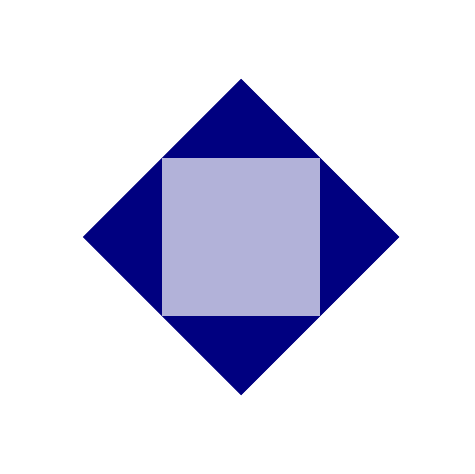
\begin{tikzpicture}[font=\small]
		\fill[main, NavyBlue] (1,-1) -- (3,1) -- (1,3) -- (-1,1) -- cycle;
		\fill[main, NavyBlue!30] (0,0) -- (2,0) -- (2,2) -- (0,2) -- cycle;
		
		\draw[main] (0,0) node [below left] {A};
		\draw[main] (2,0) node [below right] {D};
		\draw[main] (2,2) node [above right] {C};
		\draw[main] (0,2) node [above left] {B};
		
		\draw[main] (-1,1) node [left] {Q};
		\draw[main] (3,1) node [right] {S};
		\draw[main] (1,-1) node [below] {P};
		\draw[main] (1,3) node [above] {R};
	\end{tikzpicture}
\end{document}